%!TEX root = ../zeeman.tex
\subsection{Наблюдение нормального эффекта Зеемана}

Мы пронаблюдали характер поляризации компонент в поперечном эффекте, исследуя линию с  длиной волны  585.25 нм. Продольный эффект не изучался, так как на данной установке он не виден.

\begin{figure}[H]
	\centering
	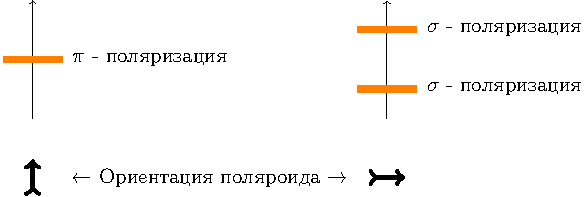
\includegraphics[scale=1]{ris/2a}
	\caption{Характер поляризации компонент}
	\label{fig:ris2a}
\end{figure}

Задав значение магнитного поля в 5520 эрстед, мы замерили расщепление линий:

\begin{figure}[H]
	\centering
	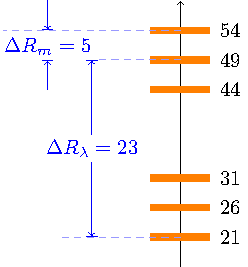
\includegraphics[scale=1]{ris/2b}
	\caption{Вид двух соседних колец интерферометра Фабри-Перо при расщеплении спектральной линии в магнитном поле в выходной плоскости спектрографа}
	\label{fig:ris2b}
\end{figure}

По формуле (\ref{eq:35}) рассчитаем $\delta\lambda$:

\begin{equation}
 	\delta \lambda=\frac{\lambda^2}{2h}\cdot\frac{5}{23}
 \end{equation} 

Здесь h=4 мм,  $\lambda$=585.25 нм:

\begin{equation}
 	\delta \lambda=\frac{585.25^2\cdot10^{-18}}{2\cdot4\cdot10^{-4}}\cdot\frac{5}{23}=9.30\cdot10^{-11} \text{ м}
 \end{equation} 

Тогда отсюда

\begin{equation}
	\Omega=\frac{2\pi c}{\lambda+\delta \lambda}-\frac{2\pi c}{\lambda-\delta \lambda}=8.41\cdot10^{10} \text{ рад/c}
\end{equation}

И в рамках классической модели (см. \ref{eq:22}), в СГС:

\begin{equation}
	\frac{e}{m}=\frac{2\Omega c}{H}=9.23\cdot10^{17}=
\end{equation}

Отметим, что табличное значение заряда к массе в СГС $5.27\cdot10^{17}$.

Оценим разрешающую способность \textbf{ИФП}. 

Теоретически мы можем рассчитать её,воспользовавшись формулой (\ref{eq:27}), подставляя туда максимальный порядок интерференции $m_0=\frac{2h}{\lambda}$: 

\begin{equation} 
R=\frac{m_0\pi\sqrt{\rho}}{1-\rho}=368299 
\end{equation} 

Экспериментальную разрешающую способность будем оценивать как: 
\begin{equation} 
R=\frac{\omega}{\Delta \omega}=28274 
\end{equation}

\subsection{Изучение аномального эффекта Зеемана}

\subsubsection{<<Квазинормальный>> случай}

Аномальный эффект исследовался в <<квазинормальном>> случае, когда в спектре представлены только три компоненты --- исследуя линию с  длиной волны  607.4 нм.

Магнитное поле H=5406 эрстед.

\begin{figure}[H]
	\centering
	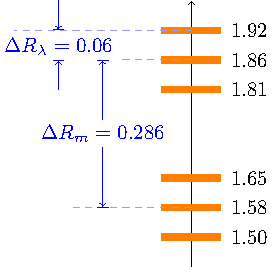
\includegraphics[scale=1]{ris/3b}
	\caption{Вид двух соседних колец интерферометра Фабри-Перо при расщеплении спектральной линии в магнитном поле в выходной плоскости спектрографа}
	\label{fig:ris3b}
\end{figure}

Теоретически посчитанное в рамках LS-приближения (\ref{eq:21}) значения  g-факторов здесь
\begin{equation}
	g_1=g_2\equiv g=1+\frac12=1.5
\end{equation}

Здесь h=4 мм,  $\lambda$=607.4 нм:

\begin{equation}
 	\delta \lambda=\frac{607.4^2\cdot10^{-18}}{2\cdot4\cdot10^{-3}}\cdot\frac{0.06}{0.286}=8.23\cdot10^{-12} \text{ м}
 \end{equation} 

Тогда отсюда

\begin{equation}
	\Omega=\frac{2\pi c}{\lambda+\delta \lambda}-\frac{2\pi c}{\lambda-\delta \lambda}=84.15\cdot10^{9} \text{ рад/c}
\end{equation}

И по формуле (\ref{eq:11}) получим

\begin{equation}
	g=\frac{\Omega \hbar}{\mu_0 H}=1.77
\end{equation}

Как видно, сходится неплохо.

% \newpage
\subsubsection{Случай наличия более трех разрешаемых компонент}

В данном эксперименте длина волны 638.3 нм, поле $H=$
\begin{figure}[h!]
	\centering
	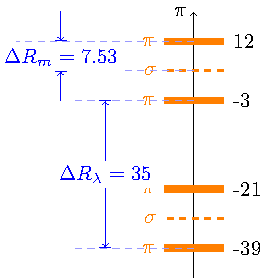
\includegraphics[scale=1]{ris/4b}
	\caption{Вид двух соседних колец интерферометра Фабри-Перо при расщеплении спектральной линии в магнитном поле в выходной плоскости спектрографа}
	\label{fig:ris4b}
\end{figure}

Рассчитаем разность g-факторов по формуле (\ref{eq:11}):

\begin{equation}
g_{1}=1+\frac{1\cdot(1+1)-1\cdot(1+1)}{2\cdot01\cdot(1+1)}=1; g_{2}=1+\frac{1\cdot(1+1)+1\cdot(1+1)-2\cdot(2+1)}{2\cdot1\cdot(1+1)}=1
\end{equation}

Так как мы смотрим $\pi$ -- компоненты, то согласно правилам отбора (стр. 7 методички) $\Delta M=0$, тогда $M_1=M_2=1$ и теоретически

\begin{equation}
	\Delta g=g_2-g_1=0.5
\end{equation}

Из эксперимента же рассчитано, по формуле (\ref{eq:11})

\begin{equation}
	\Delta g=g_2-g_1=1.89
\end{equation}


\subsubsection{Случай частичого разрешения компонент}

Мы проследили за изменением картины расщепления в широком диапазоне поля $H$ и определили характер поляризации компонент в поперечном эффекте:

\begin{figure}[h!]
	\centering
	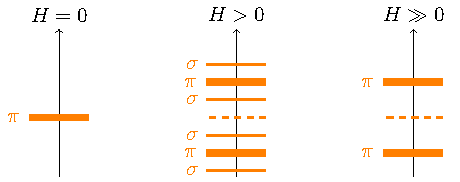
\includegraphics[scale=1]{ris/5}
	\caption{Вид двух соседних колец интерферометра Фабри-Перо при расщеплении спектральной линии в магнитном поле в выходной плоскости спектрографа}
	\label{fig:ris5}
\end{figure}
